\begin{center}
    \addcontentsline{toc}{section}{ГЛАВА 3. ПРАКТЫЧНАЯ РЭАЛІЗАЦЫЯ}
    \section*{ГЛАВА 3. \\ ПРАКТЫЧНАЯ РЭАЛІЗАЦЫЯ}
\end{center}

Рэалізацыі алгарытмаў, разгледжаных у папярэдняй главе, даступныя ў вольным доступе
як праекты з адкрытым зыходным кодам. Аўтары каментуюць публікацыю як адначасова
унёсак у SLAM супольнасць і сродак для даследчыкаў з памежных галінаў \cite{murORB2}.

У супольнасці робататэхнікаў папулярнасцю карыстаецца ROS - аперацыйная сістэма для
распрацоўкі прыкладанняў для робатаў. Праз тое, што SLAM-алгарытмы ў шматлікіх
выпадках знаходзяць прымяненне ў галіне робататэхнікі, большасць рэалізацыяў
SLAM-алгарытмаў мае падтрымку інтэрфейсаў ROS-а, а ў некаторых выпадках гэта з'яўляецца
наогул адзіным рэжымам працы.

Канечная мэта маёй працы - пабудова эфектыўнай сістэмы аўтаматычнай рэканструкцыі
трохмерных паверхняў па дадзеных з беспілотных лятальных апаратаў; у сваіх даследваннях
я рабіў упор на спалучэнне SLAM-рэалізацыяў з ``класічнымі'' падыходамі. Пры рэалізацыі я сутыкнуся
з наступнымі аспектамі, пра якія мне хацелася б распавесці ў асобных пунктах ніжэй.

\vspace{5mm}

\addcontentsline{toc}{subsection}{3.1 ROS}
\subsection*{3.1 ROS}

ROS (The Robot Operating System) - фрэймворк для напісання праграмнага забеспячэння
для робатаў, з'яўляецца наборам інструментаў, бібліятэкаў і
канвенцыяў для зручнай і надзейнай працы з робатамі (\cite{288}). Патрэбнасць у фрэймворку ўзнікла
праз той факт, што стварэнне праграмнага забеспячэння для робатаў -
вельмі складаны і шматэтапны працэс; уніфікацыя спосабу камунікацыяў паміж часткамі вялікай
сістэмы дазваляе камандам працаваць над навігацыяй, рухам і зрокам робата асобна.

ROS пабудаваны на ідэі кліент-сервернага ўзаемадзеяння, што спрашчае працу ў размеркаваных
сістэмах, хаця і можа часам падавацца залішнім пры запуску на адной лакальнай машыне.

У аснове ROS ляжаць:

\begin{itemize}
  \item нізкаўзроўневы інтэрфейс перадачы паведамленняў,
  \item ананімная і асінхронная сістэма публікацыі і падпіскі на паведамленні,
  \item магчымасць рэалізацыі RPC для сінхроннага выкліку метадаў іншых пакетаў,
  \item глабальнае сховішча ключэй і значэнняў,
  \item зручныя сродкі дыягностыкі,
  \item інструменты для працы з ROS-ам праз графічны інтэрфейс: \textit{rviz}, \textit{rqt}.
\end{itemize}

Усе гэтыя ўласцівасці ROS-а робяць распрацоўку зручнай і лёгка ўбудоўваемай ў іншыя сістэмы.
Вялікая колькасць SLAM-алгарытмаў рэалізаваныя менавіта пад ROS і могуць не мець
уласных сродкаў візуалізацыі альбо ўводу дадзеных.

Падчас рэалізацыі ўласнага праграмнага забеспячэння мне давялося шчыльна пазнаёміцца з ROS-ам
і прынцыпамі арганізацыі працы ў гэтай аперацыйнай сістэме.

\addcontentsline{toc}{subsection}{3.2 Архітэктура сістэмы}
\subsection*{3.2 Архітэктура сістэмы}

Архітэктура сістэмы, рэалізацыяй якой я займаўся, і ўсе яе ключавыя вузлы схематычна
прадстаўленыя на малюнку \ref{fig:architecture}.

\begin{figure}[H]
  \centering
  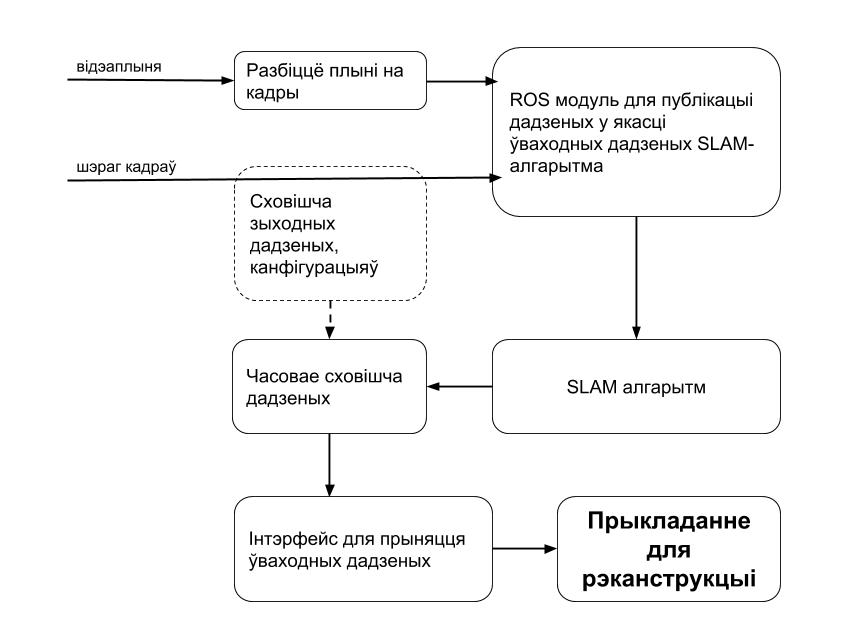
\includegraphics[width=\textwidth]{architecture}
  \captionsetup{labelformat=empty}
  \caption{Малюнак \arabic{figure}: архітэктура спалучанай сістэмы}
  \label{fig:architecture}
\end{figure}

Тут і далей, \textit{Appa} (\cite{appa-software}) - праграмнае забеспячэнне для рэканструкцыі
паверхні па зыходных дадзеных у выглядзе набора малюнкаў. Распрацоўка праграмы пачалася
ў межах курсавой працы і працягваецца зараз. Асноўныя магчымасці праграмы: выманне ключавых кропак,
ажыццяўленне пошуку адпаведнасцяў, рэканструкцыя паверхні, нанясенне колераў, праца з праектамі,
падтрымка шматлікіх мадэляў у межах аднаго праекта. \textit{Appa} добра спраўляецца з
утрыманнем вялікай колькасці параметраў і опцыяў; праекты Appa лёгка пераносяцца паміж сістэмамі.

\addcontentsline{toc}{subsection}{3.3 Тыпы ўваходных інтэрфейсаў}
\subsection*{3.3 Тыпы ўваходных інтэрфейсаў}

У сваёй сістэме, як бачна на малюнку \ref{fig:architecture}, я дадаў падтрымку двух інтэрфейсаў для ўводу дадзеных.

Першы - перанакіраванне відэаплыні наўпрост з вэб-камеры ці любой іншай сістэмы захопу відэа.
У такім рэжыме мы найбольш набліжаемся да ўмоваў, якія можа сустрэць алгарытм пры запуску на
лятальным апараце пры выкананні рэальнага палёту.

Другі - больш ``лабараторны'' - публікацыя паслядоўнасці кадраў загадзя падрыхтаванага
набора дадзеных. Такі рэжым значна лепш падыходзіць для тэставання і адладкі алгарытма
і дае магчымасць паўтараць эксперыменты на аднолькавых дадзеных.

Падтрымка абодвух рэжымаў стала магчымай праз напісанне ўласных утылітаў для ROS
альбо мадыфікацыю існуючых. Трэба дадаць, што на наступных этапах мы працуем
з дадзенымі як з мноствам кадраў альбо выяваў - такім чынам, пры наяўнасці відэаплыні
на ўваходзе ўзнікае патрэба ў разбіцці плыні на кадры з вызначанай частатой, захаванне кадраў
у форме асобнага датасэту, а таксама сінхранізацыя пазіцыяў камер з абранымі кадрамі з пачатковай
відэаплыні.

\addcontentsline{toc}{subsection}{3.4 Выманне дадатковых дадзеных са SLAM-алгарытмаў}
\subsection*{3.4 Выманне дадатковых дадзеных са SLAM-алгарытмаў}

Адным з найбольш крытычных месцаў працы сістэмы з'яўляецца выманне ўсіх патрэбных нам дадзеных
са SLAM-алгарытмаў і узгадненне гэтага фармату дадзеных, для паспяховага пераходу да
наступных крокаў.

Першае, што варта тут згадаць - патрэбныя нам дадзеныя не выдаюцца алгарытмамі ў гатовым выглядзе.
У якасці выходных дадзеных нас найбольш цікавіць граф узаемабачнасці кропак з камераў
(\textit{covisibility graph}) - граф, вяршынямі якога з'ўляюцца камеры (альбо ключавыя кадры), рэбры
праводзяцца паміж тымі вяршынямі, адпаведныя камеры якіх маюць дастаткова вялікую агульную
аглядную прастору (вымяраецца ў колькасці знойдзеных агульных трохмерных кропак). Таксама
цікаўнасць прадстаўляюць ацэнкі пазіцыяў камер, якія можна альбо прыняць за ісціну, альбо
скарыстаць у якасці апрыорнай ацэнкі. Патрэба ва ўсіх гэтых дадзеных прымушае нас
разбіраць той ці іншы SLAM-алгарытм на кавалкі, шукаць патрэбныя дадзеныя у кодзе і знаходзіць магчымасці
выгрузкі іх у вонкавы сусвет.

Па-другое, працуючы з рознымі SLAM-алгарытмамі, мы павінны падыходзіць да кожнага з іх
індывідуальна, шукаючы магчымасць выгрузіць патрэбныя нам дадзеныя, але, ў выніку,
прадставіць дадзеныя ва ўніфікаванай форме, незалежнай ад выкарыстанага SLAM-алгарытма.
Індывідуальная праца з кожным асобна ўзятым алгарытмам досыць моцна ўскладняе нашую задачу.

\addcontentsline{toc}{subsection}{3.5 Appa і інтэрфейс для дадзеных са SLAM-а}
\subsection*{3.5 Appa і інтэрфейс для дадзеных са SLAM-а}

У межах пераддыпломнай практыкі я працягнуў працу над праграмным забеспячэннем
для рэканструкцыі паверхні па здымках з беспілотных лятальных апаратаў \textit{Appa} \cite{appa-software},
працу над якім я пачаў раней у межах курсавой працы.

\begin{figure}[H]
  \centering
  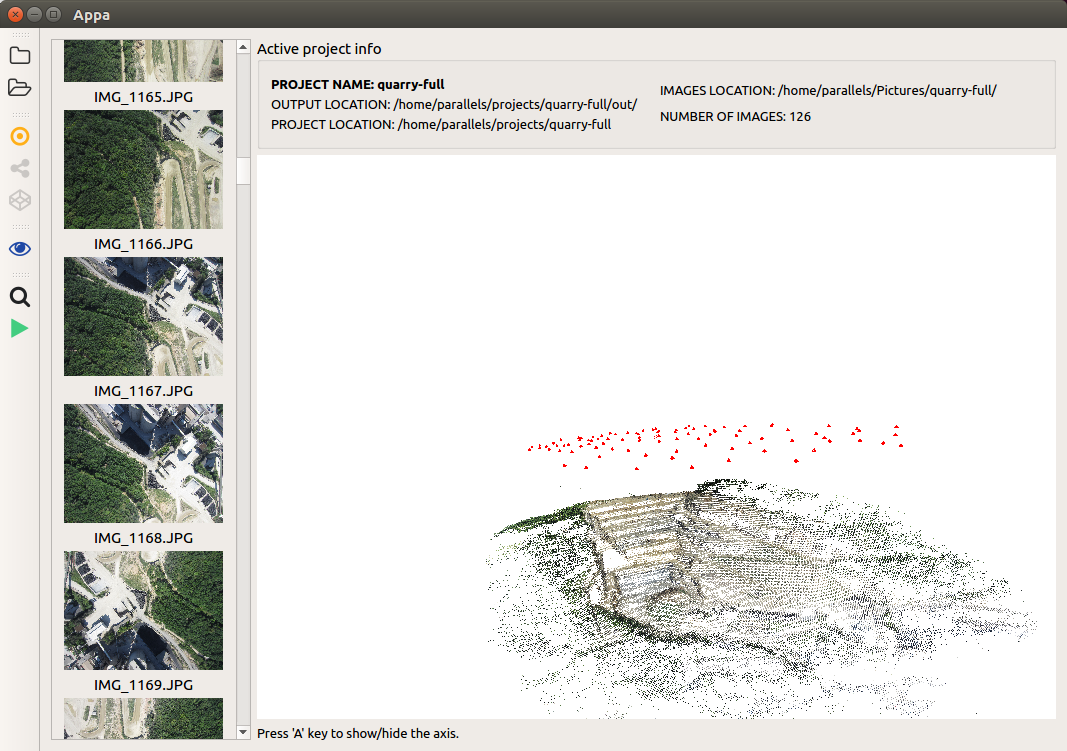
\includegraphics[width=\textwidth]{appa0}
  \captionsetup{labelformat=empty}
  \caption{Малюнак \arabic{figure}: праграмнае забеспячэнне для трохмернай рэкаструкцыі Appa}
  \label{fig:appa0}
\end{figure}

Першасныя ўдасканальванні, якія патрабуе \textit{Appa} - распрацоўка інтэрфейса, які б
даваў магчымасць ўводзіць дадзеныя, сабраныя на папярэдніх этапах працы сістэмы. З ростам аб'ёмаў
дадзеных да інтэрфейсу ўводу прад'яўляюцца ўсё больш жорсткія патрабаванні да хуткасці працы,
што прымушае шукаць больш дасканалыя структуры дадзеных для часовага захавання графа ўзаемабачнасці
з усімі патрэбнымі дадатковымі параметрамі.

\addcontentsline{toc}{subsection}{3.6 Аптымізацыя камунікацыяў з дапамогай ROS-а}
\subsection*{3.6 Аптымізацыя камунікацыяў з дапамогай ROS-а}

Яшчэ адным накірункам маёй працы ёсць аптымізацыя камунікацыяў паміж часткамі
сістэмы. У папярэдніх пунктах у асноўным апісваліся камунікацыі праз файлавую сістэму - камунікацыі могуць быць
аптымізаваныя з дапамогай убудаваных сродкаў камунікацыяў у ROS: публікацыя ў ROS-аўскі
``topic'' з аднаго боку і праслухоўванне з іншага з'яўляецца, у агульным
выпадку, значна больш дасканалым спосабам злучэння асобных элементаў сістэмы з малюнку \ref{fig:architecture}
у адно суцэльнае. Гэты спосаб таксама дазваляе паскорыць камунікацыі,
бо абмен дадзенымі ідзе праз RAM-памяць замест файлавай сістэмы.

\newpage
